\chapter{Evaluation}
\label{evaluation}
This chapter covers the evaluation of the work by describing the implementation of a smaller tokenization contract in order to show an example of the possible functionality and by providing the implementation of a modular exponentiation contract. The modular exponentiation contract is set in comparison with a Go program in order to show the overhead created by the execution of the logic on the Bazo VM.

\section{Tokenization Contract}
\label{tokencontract}
Tokenization is the process of recording the rights to an asset as a digital token on a blockchain in the form of sub-currencies. \cite{eth_whitepaper} Tokenization is the first use-case for smart contracts that has found wide application. New possibilities for funding start-ups and companies have emerged in the form of initial coin offerings (ICOs) also known as token sales. The tokens of an ICO can be bought by sending money in the form of the blockchain currency to a smart contract. The investor then receives corresponding amount in tokens. Ideally, the token is an integral component within the ecosystem of the company hosting the ICO. \cite{ico_pwc} Since tokenization contracts have become so widely used and because they are generally simple, since they do not need to interact with off-chain data, it was decided to write a tokenization contract. In the very basic implementation, a tokenization contract consists of a map of account addresses and balances and methods to transfer those tokens from one account to another.

 \begin{minted}	[
frame=lines,
framesep=2mm,
baselinestretch=1.2,
fontsize=\footnotesize,
linenos
]
{yaml}
CALLDATA
# ------- ABI -------------------------
DUP
PUSH 1
EQ
CALLIF mint 3
HALT

# ------ Contract ---------------------
mint:
LOAD 1 # load value
LOAD 0 # load key
SLOAD 1 # load address of minter
CALLER
EQ
CALLIF adjustBalance 2
RET

adjustBalance:
LOAD 1 # load value
LOAD 0 # load key
DUP
SLOAD 2 # load map
MAPHASKEY
CALLIF addKeyIfNotExists 2
LOAD 1 # load value
LOAD 0 # load key
SLOAD 2 # load map
MAPPUSH
SSTORE 2 # store the map
HALT

addKeyIfNotExists:
LOAD 1 # load key
SLOAD 2 # load map
MAPGETVAL
LOAD 0 # load value
ADD
LOAD 1 # load key
SLOAD 2  # load map
MAPSETVAL
SSTORE 2 # store the map
HALT
\end{minted}

\subsection{Results}
As a result, a contract was created which allows to store addresses together with balances. Only the account address which is recorded as minter is allowed to change balances. The balance can be reduced by sending negative values or increased by sending positive values. If the map does not yet contain an address, it is added automatically.

\section{Benchmarking Contract}
The performance of the virtual machine is crucial for the speed of execution and the blockchain in general. For this reason a smart contract has been developed which is suitable for comparing the speed of execution on different implementations and platforms. Taking into consideration that blockchains and its use-cases depend heavily on public-key cryptographic, it was decided to implement a smart contract which performs modular exponentiation. Modular exponentiation is a one-way function and frequently used in cryptography. Figure \ref{mod_exp_direct} shows the straightforward method to calculate \textit{c}.

\begin{figure}[thp]%
    	\centering
		$
		c\quad \equiv \quad { b }^{ e }\quad mod\quad m
		$
		\caption{Modular exponentiation straightforward method}
		\label{mod_exp_direct}
\end{figure}

Considering \textit{b} is at least 256 bits for strong cryptography, this method is not very efficient. Therefore, a more memory efficient method has been implemented, which is shown in figure \ref{modularPow_pseudocode}. The benchmarking function has been implemented as a Go program and as a contract in \flqq Bazo Byte Code\frqq. The main goal is to compare the overhead.

\begin{figure}[thp]%
    	\centering
		\begin{minipage}{0.7\textwidth}
		\begin{minted}
		[
		frame=lines,
		autogobble,
		framesep=2mm,
		baselinestretch=1.2,
		fontsize=\footnotesize,
		linenos
		]{python}
function modular_pow(base, exponent, modulus)
    if modulus = 1 then return 0
    c := 1
    for e_prime = 0 to exponent-1
        c := (c * base) mod modulus
    return c
		\end{minted}
		\caption{Memory efficient method to compute modular exponentiation}
		\label{modularPow_pseudocode}
		\end{minipage}
\end{figure}

\subsection{Results}
The Go testing package contains a subset of functions to measure the performance of Go code. A benchmark function runs the code \textit{b.N} times. \textit{b.N} is adjusted during execution, until the benchmark function can be timed reliably. \cite{golang_testing} Three benchmark functions for both, the Go program and the contract, have been implemented, whose only difference is the length of \textit{b}. The length of \textit{b} is 32 bytes in the first benchmark function, which is the minimum length for strong cryptography. In the second benchmark function the length of \textit{b} is 128 bytes and in the last, \textit{b} has a length of 255 bytes, which is the maximum length the virtual machine can process. The values of \textit{b}, \textit{e} and \textit{m} are random generated every run. The benchmarks have been measured on a Fujitsu Celsius W530, with 15.6 GiB RAM, an Intel Xeon CPU E3-1245 v3 \@ 3.40GHz x 8 processor, running Ubuntu 17.10 as operating system. The following benchmarking measurements have been analyzed.

\begin{tabular}[t]{ p{3cm} p{12.5cm}}
\raggedright
\textbf{Nanoseconds per operation} &
Figure \ref{nperop} shows how many nano seconds the operation took. Operation describes the code that was run, in this case the Go program and the benchmarking contract. The benchmarking contract took 9.41 times more nano seconds than the Go program in the first benchmark function with \textit{b = 32 bytes}. In the second function with \textit{b = 128 bytes}, the factor was 7.24. In the last function with \textit{b = 255 bytes} this factor went down to 5.89. The conclusion is, that the longer \textit{b} is, the better the performance of the benchmarking contract gets, compared to the program written in Go. \\ \\
\end{tabular}

\begin{figure}[H]
	\begin{center}
	\fbox{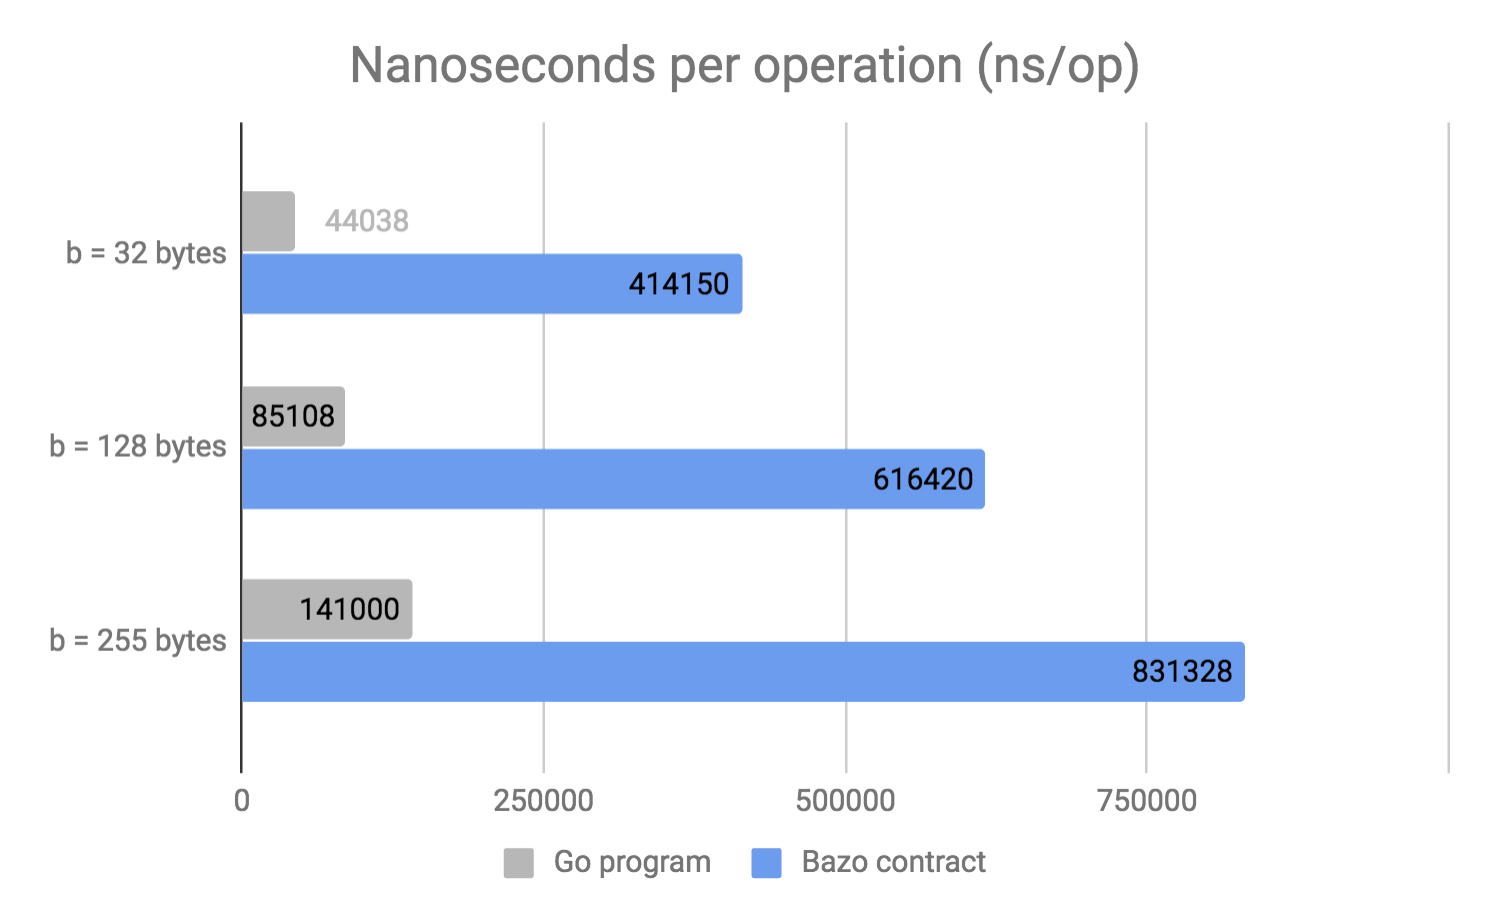
\includegraphics[width=0.6\textwidth]{./images/Benchmarking_Table_-_nsop}}
	\caption{Nanoseconds per operation diagram}
	\label{nperop}
	\end{center}
\end{figure}

\begin{tabular}[t]{ p{3cm} p{12.5cm}}
\raggedright
\textbf{Bytes per operation} &
Figure \ref{bperop} shows how many bytes per operation have been allocated. The factor between the Go program and the benchmarking contract was stable during benchmark functions. The benchmarking contract needs about 10 times more bytes. This result was expected, since the benchmarking contract needs to duplicate and roll values often, to permute a loop. \\ \\
\end{tabular}

\begin{figure}[H]
	\begin{center}
	\fbox{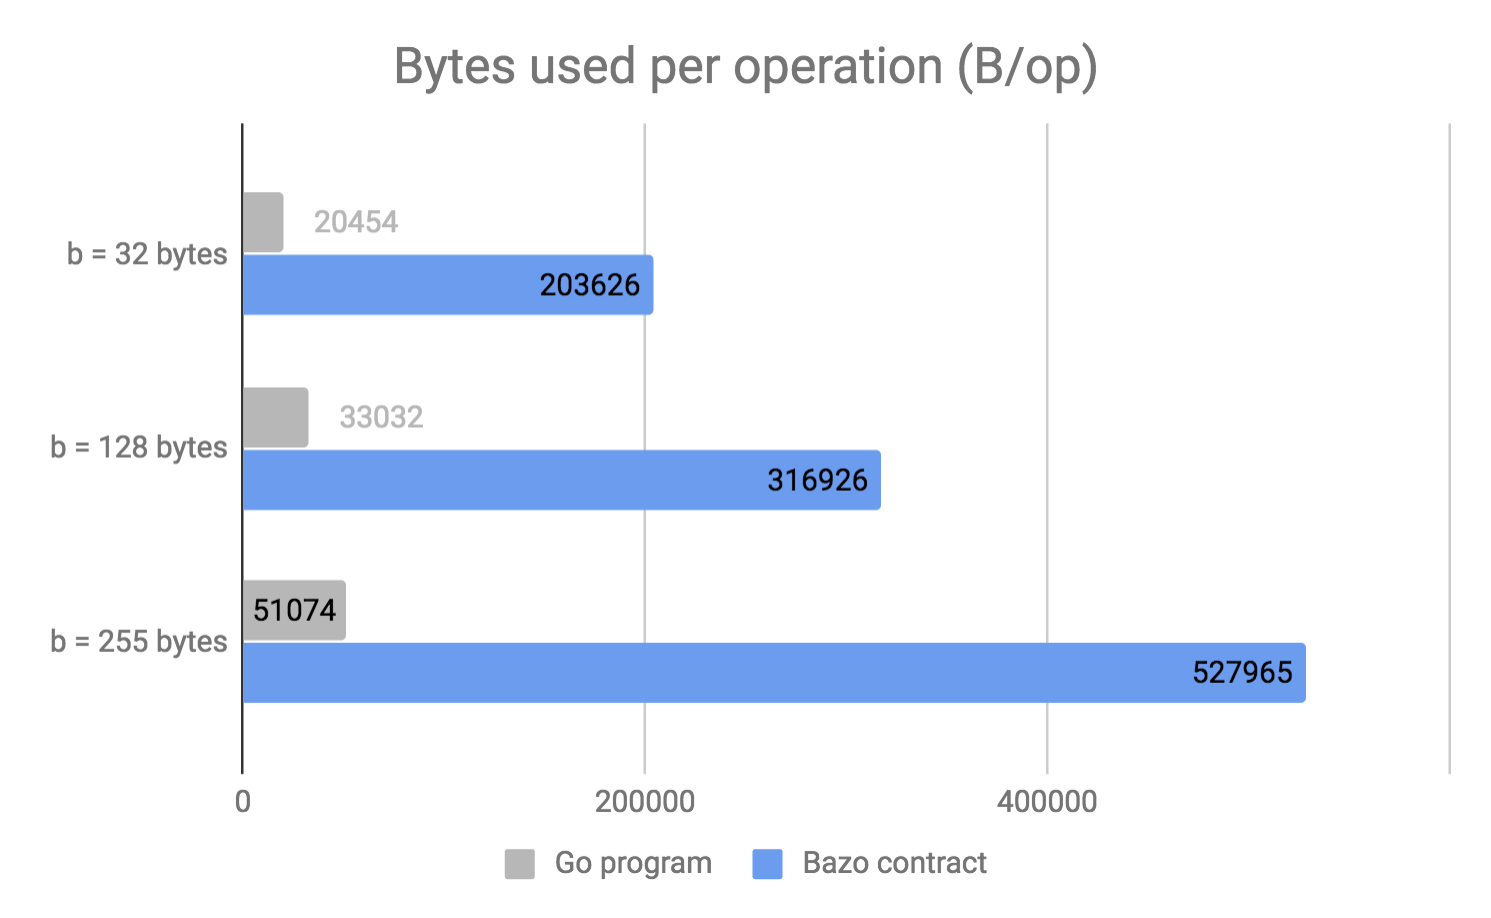
\includegraphics[width=0.6\textwidth]{./images/Benchmarking_Table_-_bop}}
	\caption{Bytes per operation diagram}
	\label{bperop}
	\end{center}
\end{figure}

\begin{tabular}[t]{ p{3cm} p{12.5cm}}
\raggedright
\textbf{Allocations per operation} &
Figure \ref{aperop} shows how many bytes per operation have been allocated. The factor between the Go program and the benchmarking contract was stable in all benchmarks. The benchmarking contract needs about 10 times more bytes. This result was expected, for the same reason mentioned above. \\ \\
\end{tabular}

\begin{figure}[H]
	\begin{center}
	\fbox{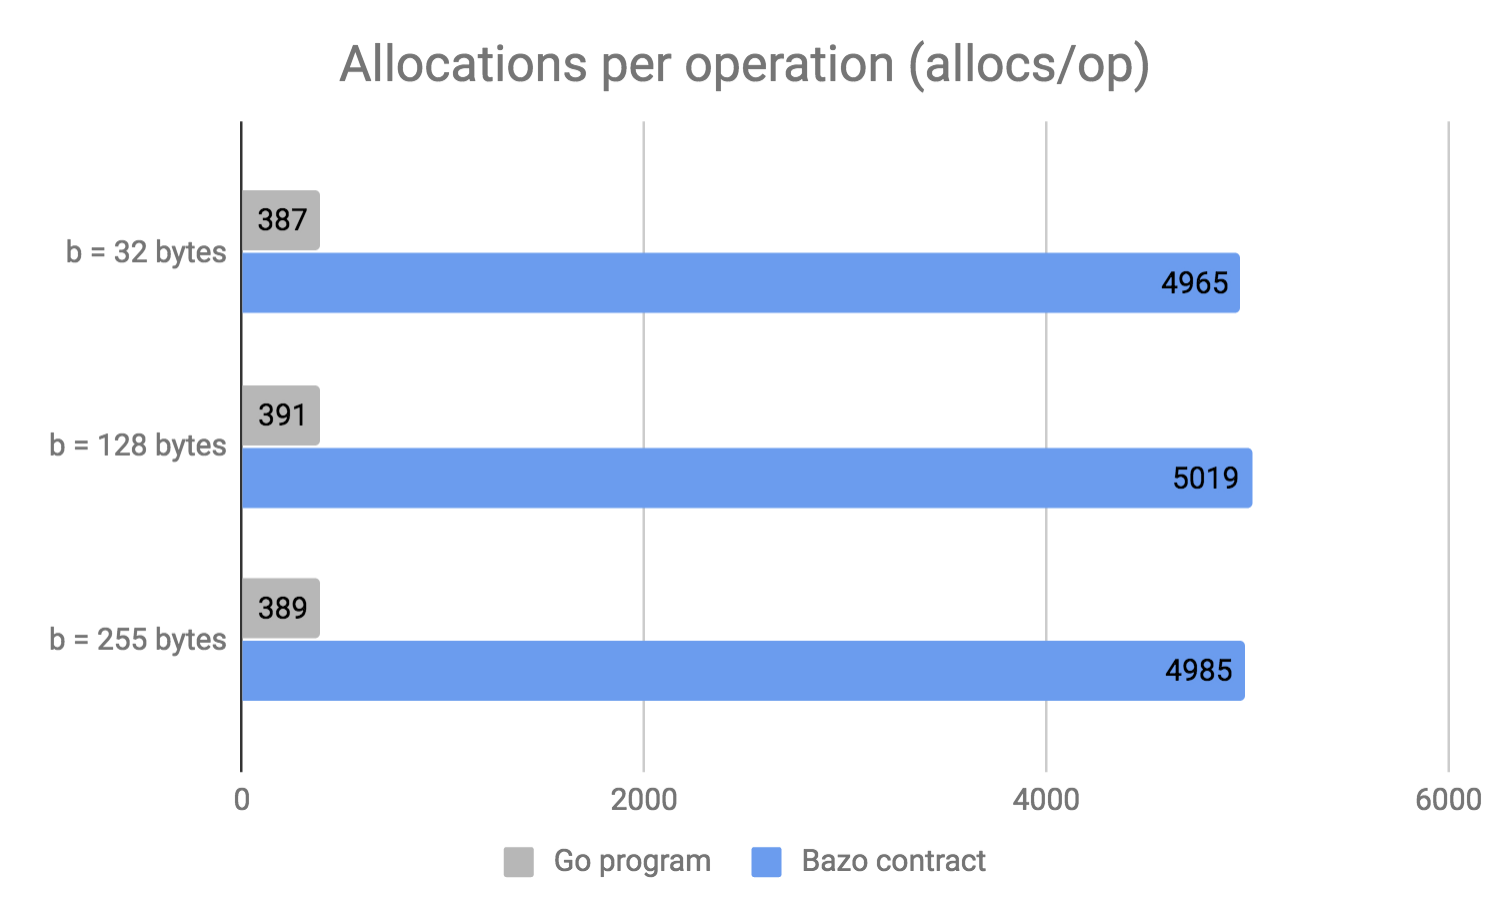
\includegraphics[width=0.6\textwidth]{./images/Benchmarking_Table_-_aop}}
	\caption{Allocation per operation diagram}
	\label{aperop}
	\end{center}
\end{figure}
